\renewcommand{\arraystretch}{1.5}
\begin{CJK*}{UTF8}{gbsn}
\begin{figure}[h]
  \centering
  \begin{tabular}{m{15cm}}
  \toprule
  \textbf{Input image:}
  \begin{center}
  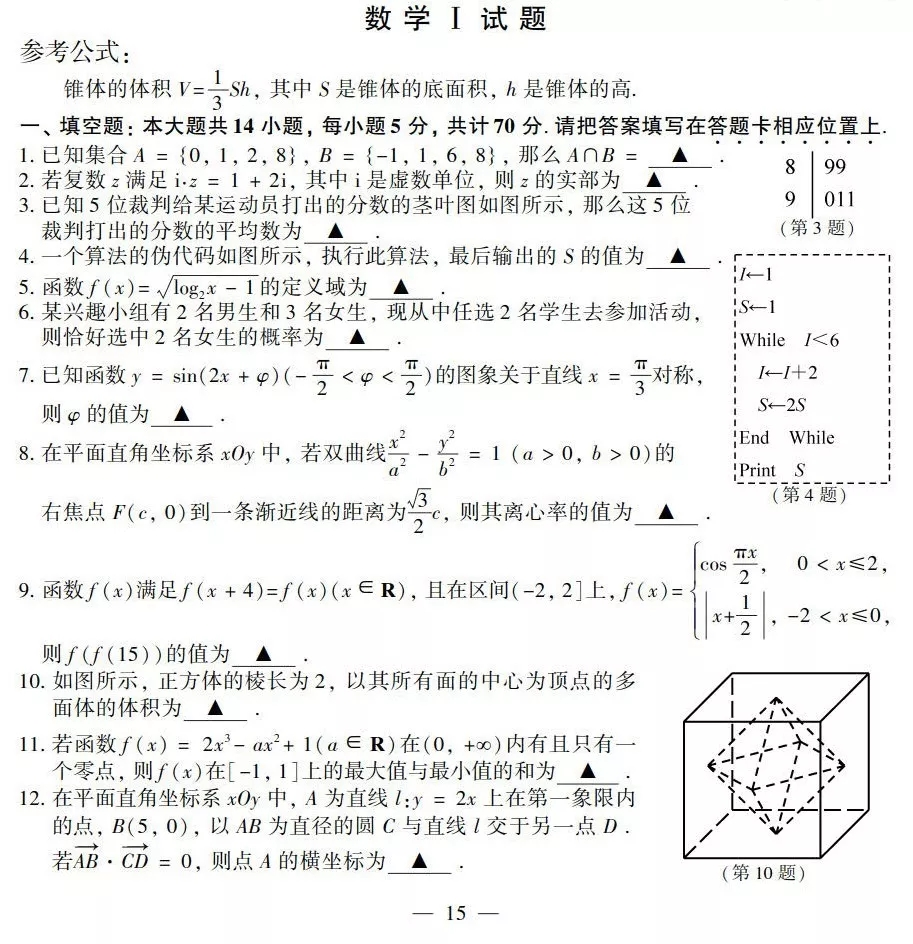
\includegraphics[width=7cm]{figures/example/example1.jpg}
  \end{center}
  \\
  {\footnotesize \textbf{Instruction:} 完成该试卷\newline\newline
  \textbf{\mimovl{}:} \texttt{<think>...</think>}
  
    \textbf{第1题：集合的交集}
    集合 $ A = \{0, 1, 2, 8\} $，$ B = \{-1, 1, 6, 8\} $，交集为同时属于两个集合的元素，即 $ A \cap B = \{1, 8\} $。  
    
    
    \textbf{第2题：复数的实部} 
    设 $ z = x + yi $（$ x, y $ 为实数），由 $ i \cdot z = 1 + 2i $，即 $ i(x + yi) = -y + xi = 1 + 2i $。  
    分离实部和虚部：$ -y = 1 $（实部），$ x = 2 $（虚部）。故 $ z $ 的实部为 $ 2 $。  
    
    
    \textbf{第3题：茎叶图的平均数}  
    茎叶图中，茎为十位，叶为个位。分数为 $ 89, 89, 90, 91, 91 $（共5个）。  
    平均数为 $ \frac{89 + 89 + 90 + 91 + 91}{5} = \frac{450}{5} = 90 $。  
    
    
    \textbf{第4题：伪代码的循环结果}
    初始化 $ I = 1 $，$ S = 1 $。循环条件 $ I < 6 $：  
    - 第1次循环：$ I = 1 + 2 = 3 $，$ S = 2 \times 1 = 2 $；  
    - 第2次循环：$ I = 3 + 2 = 5 $，$ S = 2 \times 2 = 4 $；  
    - 第3次循环：$ I = 5 + 2 = 7 $（不满足 $ I < 6 $，退出循环）。  
    最终 $ S = 8 $。  
    
    
    \textbf{第5题：函数的定义域}
    函数 $ f(x) = \sqrt{\log_2 x - 1} $ 需满足：  
    1. 二次根式内非负：$ \log_2 x - 1 \geq 0 $；  
    2. 对数有定义：$ x > 0 $。  
    由 $ \log_2 x \geq 1 $ 得 $ x \geq 2^1 = 2 $，故定义域为 $ [2, +\infty) $。  
    
    
    \textbf{第6题：组合的概率}
    2男3女中选2人，总选法 $ C_5^2 = 10 $；选中2女生的选法 $ C_3^2 = 3 $。  
    概率为 $ \frac{3}{10} $。  
    
    
    \textbf{第7题：正弦函数的对称轴}
    函数 $ y = \sin(2x + \varphi) $ 关于 $ x = \frac{\pi}{3} $ 对称，即 $ 2 \cdot \frac{\pi}{3} + \varphi = k\pi + \frac{\pi}{2} $（$ k \in \mathbb{Z} $）。  
    取 $ k = 0 $，得 $ \varphi = -\frac{\pi}{6} $（满足 $ -\frac{\pi}{2} < \varphi < \frac{\pi}{2} $）。  
    
    
    \textbf{第8题：双曲线的离心率}
    双曲线 $ \frac{x^2}{a^2} - \frac{y^2}{b^2} = 1 $，右焦点 $ F(c, 0) $（$ c = \sqrt{a^2 + b^2} $），渐近线 $ bx - ay = 0 $。  
    焦点到渐近线的距离为 $ \frac{|bc|}{\sqrt{a^2 + b^2}} = b $，由题设 $ b = \frac{\sqrt{3}}{2}c $。  
    结合 $ c^2 = a^2 + b^2 $，得 $ a = \frac{c}{2} $，离心率 $ e = \frac{c}{a} = 2 $。  
    
    
    \textbf{第9题：周期函数与复合函数}
    $ f(x + 4) = f(x) $ 说明周期为4。  
    - $ f(15) = f(15 - 4 \times 3) = f(3) = f(-1) $（$ 3 = -1 + 4 $）；  
    - $ x \in (-2, 0] $ 时，$ f(-1) = |-1 + \frac{1}{2}| = \frac{1}{2} $；  
    - $ f(\frac{1}{2}) = \cos\left( \frac{\pi}{2} \cdot \frac{1}{2} \right) = \cos\frac{\pi}{4} = \frac{\sqrt{2}}{2} $（$ \frac{1}{2} \in (0, 2] $）。  
    
    
    \textbf{第10题：多面体的体积}
    正方体棱长2，面中心坐标为 $ (\pm 1, 0, 0), (0, \pm 1, 0), (0, 0, \pm 1) $，构成正八面体。  
    正八面体体积为两个四棱锥之和，底面正方形边长 $ \sqrt{2} $，高1，体积为 $ 2 \times \frac{1}{3} \times 2 \times 1 = \frac{4}{3} $。  
    
    
    \textbf{第11题：函数的极值与零点}
    函数 $ f(x) = 2x^3 - ax^2 + 1 $ 在 $ (0, +\infty) $ 内有且只有一个零点，导数 $ f'(x) = 6x^2 - 2ax $，临界点 $ x = 0 $ 和 $ x = \frac{a}{3} $。  
    当 $ f(\frac{a}{3}) = 0 $ 时（极小值为0，仅1个零点），解得 $ a = 3 $。  
    $ f(x) $ 在 $ [-1, 1] $ 上，$ f(0) = 1 $（最大值），$ f(-1) = -4 $（最小值），和为 $ 1 + (-4) = -3 $。  
    
    
    \textbf{第12题：向量垂直的条件}
    设 $ A(x, 2x) $，$ AB = (5 - x, -2x) $，圆心 $ C\left( \frac{x + 5}{2}, x \right) $，另一交点 $ D(1, 2) $（由圆与直线交点唯一性得）。  
    向量 $ \overrightarrow{CD} = \left( \frac{-x - 3}{2}, 2 - x \right) $，由 $ \overrightarrow{AB} \cdot \overrightarrow{CD} = 0 $，解得 $ x = 3 $。  
    
    
    \textbf{答案}
    
    1. $ \boldsymbol{\{1, 8\}} $  
    2. $ \boldsymbol{2} $  
    3. $ \boldsymbol{90} $  
    4. $ \boldsymbol{8} $  
    5. $ \boldsymbol{[2, +\infty)} $  
    6. $ \boldsymbol{\frac{3}{10}} $  
    7. $ \boldsymbol{-\frac{\pi}{6}} $  
    8. $ \boldsymbol{2} $  
    9. $ \boldsymbol{\frac{\sqrt{2}}{2}} $  
    10. $ \boldsymbol{\frac{4}{3}} $  
    11. $ \boldsymbol{-3} $  
    12. $ \boldsymbol{3} $
    }
  \\
  \bottomrule
  \end{tabular}
\caption{Example of \mimovlrl{} answering all questions within a whole test paper.}
\label{fig:case1}
\end{figure}
\renewcommand{\arraystretch}{1}
\end{CJK*}
\clearpage
